\documentclass[12pt]{article}
\usepackage{mathematics}

\begin{document}

\title{Oxford M2 - Real Analysis I - Sequences and Series
  \footnotetext{\url{https://courses.maths.ox.ac.uk/node/37482}}} \author{Dan Davison}
\author{}
\date{}
\maketitle

\section{Sheet 1}

\newpage
\subsection{}
\begin{mdframed}
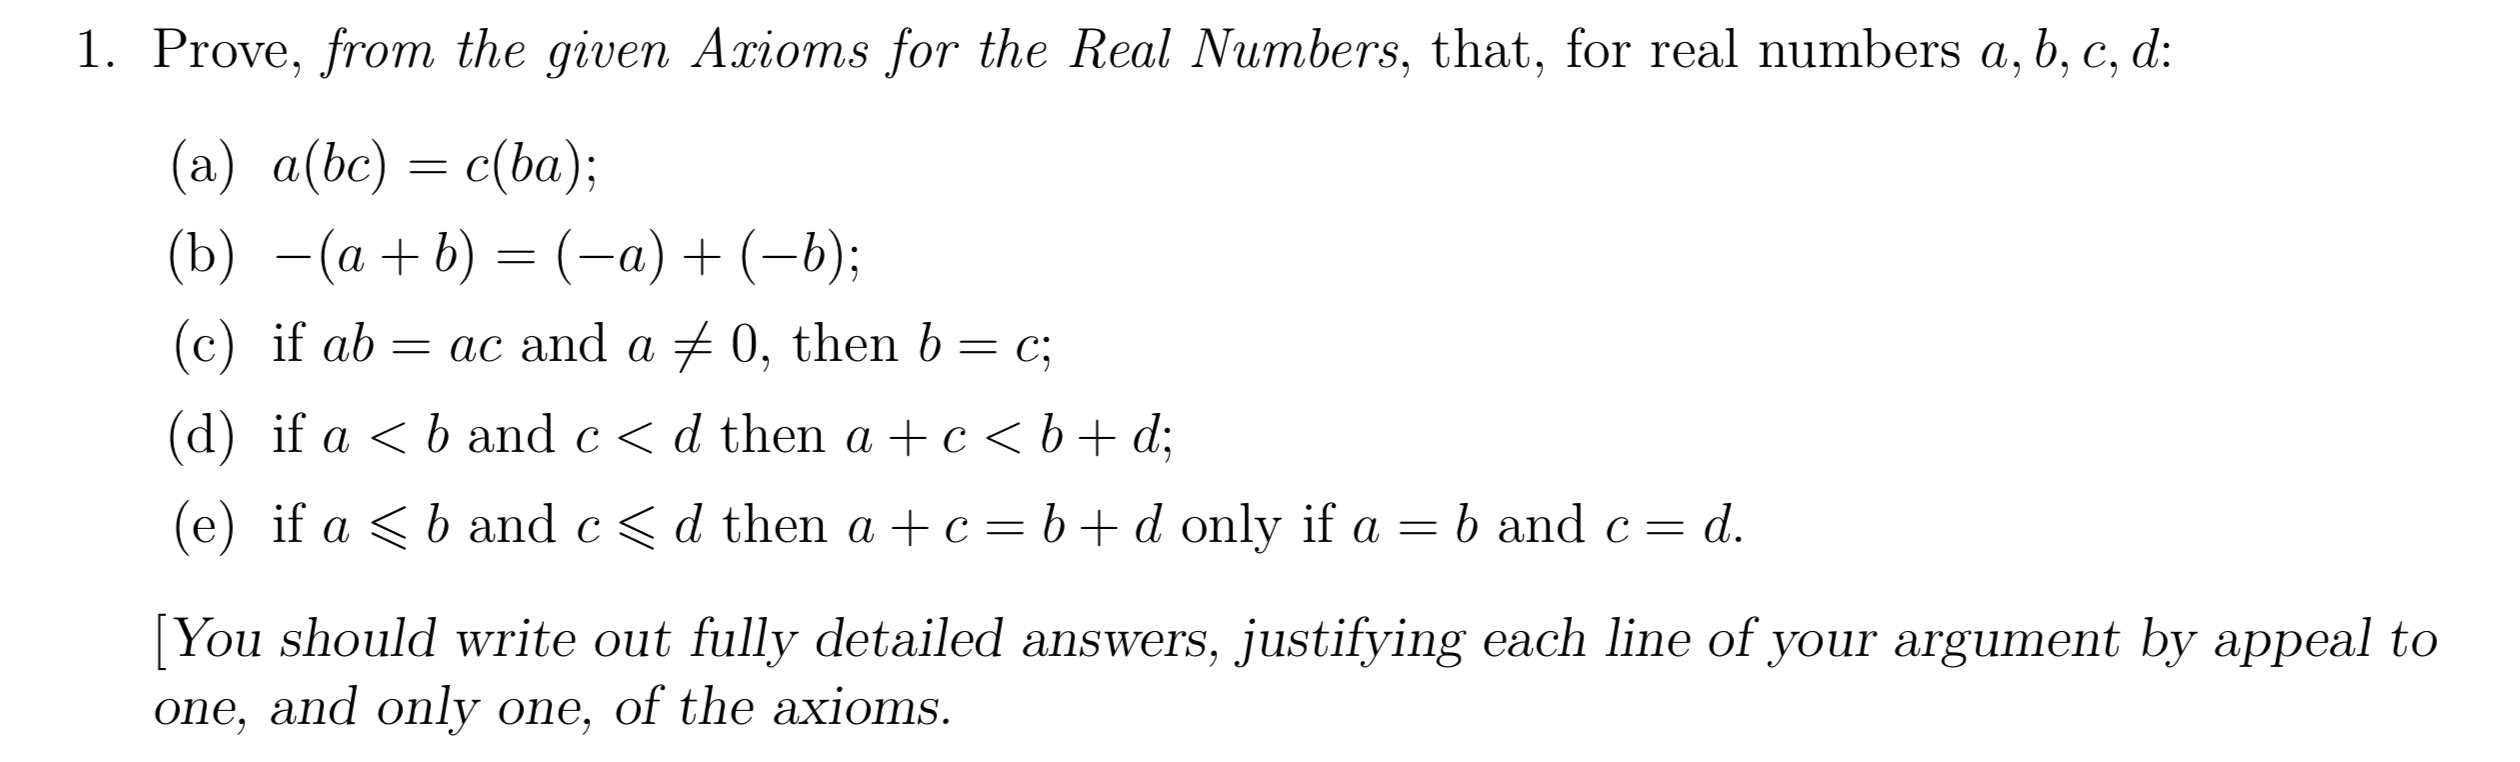
\includegraphics[width=400pt]{img/oxford-M2-analysis-I-1-1.png}
\end{mdframed}

\begin{enumerate}[label=(\alph*)]
\item \begin{theorem*} $a(bc) = c(ba)$\end{theorem*}
  \begin{proof}
    \begin{align*}
      a(bc) &= a(cb)  ~~~~~~~ \text{(M1 commutativity of multiplication)}\\
            &= (ac)b  ~~~~~~~ \text{(M2 associativity of multiplication)}\\
            &= (ca)b  ~~~~~~~ \text{(M1 commutativity of multiplication)}\\
            &= c(ab)  ~~~~~~~ \text{(M2 associativity of multiplication)}\\
            &= c(ba)  ~~~~~~~ \text{(M1 commutativity of multiplication)}
    \end{align*}
  \end{proof}
\item
  \begin{theorem*}
    $-(a + b) = (-a) + (-b)$
  \end{theorem*}
  \begin{proof}
    \begin{align*}
      (a + b) + (-(a + b))                   &= 0           ~~~~~~~ \text{definition of negative}\\
      \Big((-a) + (-b)\Big) + \Big((a + b) + (-(a + b))\Big) &= (-a) + (-b) ~~~~~~~ \text{add to both sides what axiom is this?}\\
      \Big((-b) + (-a)\Big) + \Big((a + b) + (-(a + b))\Big)   &= (-a) + (-b) ~~~~~~~ \text{S1 commutativity of sum}\\
      \Big(((-b) + (-a)) + (a + b)\Big) + (-(a + b))   &= (-a) + (-b) ~~~~~~~ \text{S2 associativity of sum}\\
      \Big((-b) + ((-a) + a) + b)\Big) + (-(a + b))    &= (-a) + (-b) ~~~~~~~ \text{S2 associativity of sum}\\
      \Big((-b) + (0 + b)\Big) + (-(a + b))            &= (-a) + (-b) ~~~~~~~ \text{definition of negative}\\
      \Big((-b) + b\Big) + (-(a + b))                &= (-a) + (-b) ~~~~~~~ \text{definition of 0}\\
      0 + (-(a + b))                         &= (-a) + (-b) ~~~~~~~ \text{definition of negative}\\
      -(a + b)                               &= (-a) + (-b) ~~~~~~~ \text{definition of 0}\\
    \end{align*}
  \end{proof}
\end{enumerate}

\newpage
\subsection{}
\begin{mdframed}
  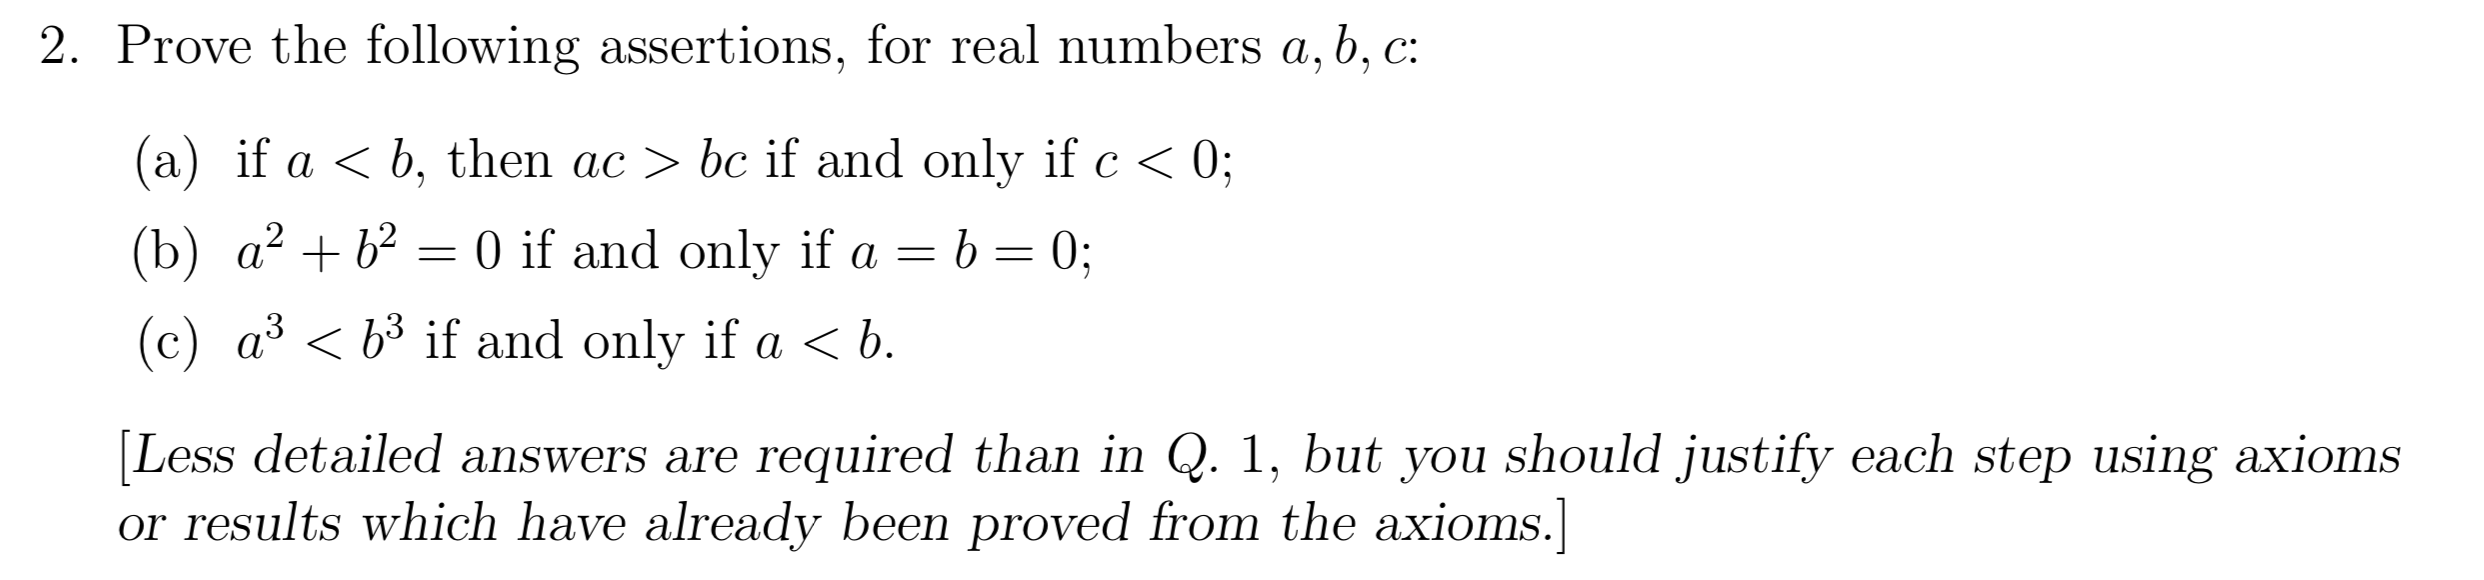
\includegraphics[width=400pt]{img/oxford-prelims-M2-analysis-I-sheet-1-2.png}
\end{mdframed}

\begin{enumerate}[label=(\alph*)]
\item
  \begin{theorem*}
    If $a < b$ then $ac > bc$ iff $c < 0$.
  \end{theorem*}
  \begin{intuition*}
    Multiplication by a scalar flips orientation iff the scalar is negative.
  \end{intuition*}
  \begin{proof}~\\
    \red{TODO} Prove carefully being explicit about which axioms are used.\\
    Let $\P$ be the strictly positive reals. We have $a < b$, i.e. $b - a \in \P$.\\
    $\implies$:\\
    We have $ac > bc$ i.e. $ac - bc \in \P$.

    Therefore
    \begin{align*}
      (a - b)c &\in \P\\
      (b - a)(-c) &\in \P\\
      \frac{1}{b-a}(b - a)(-c) &\in \P\\
      (-c) &\in \P
    \end{align*}

    $\impliedby$:\\
    We have $c < 0$, i.e. $-c \in \P$. Therefore $(-c)(b - a) \in \P$ (by {\bf P2}). Therefore
    $ac - bc \in \P$, i.e. $ac > bc$.
  \end{proof}
\end{enumerate}~\\

\newpage
\subsection{}
\begin{mdframed}
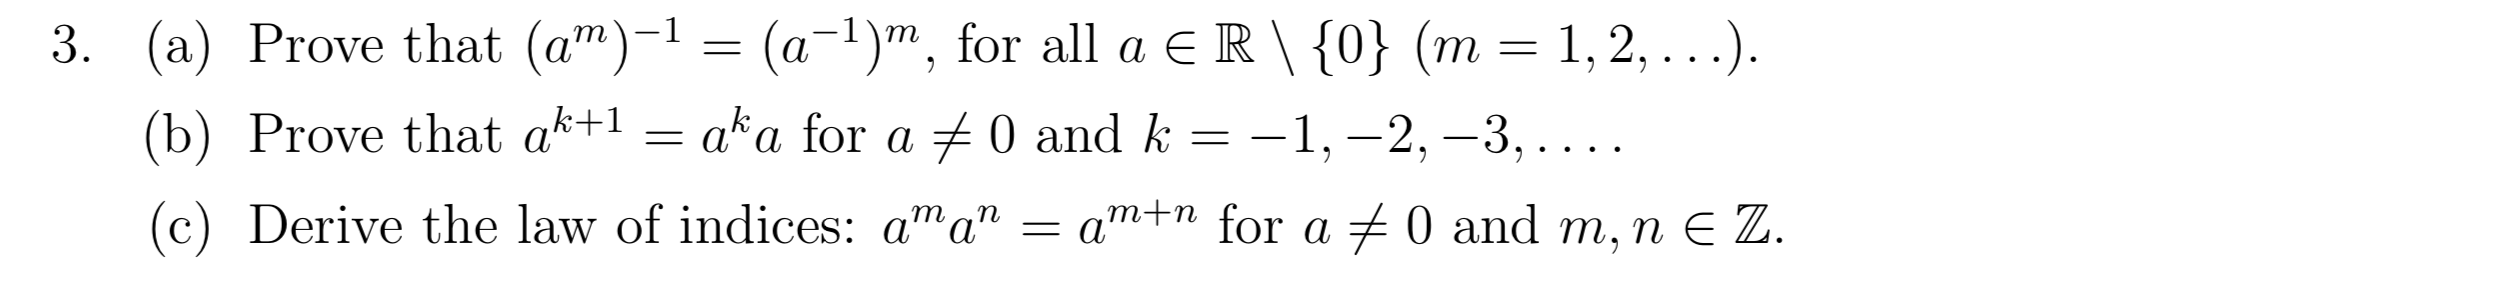
\includegraphics[width=400pt]{img/oxford-prelims-M2-analysis-I-sheet-1-3.png}
\end{mdframed}
\newpage
\subsection{}
\begin{mdframed}
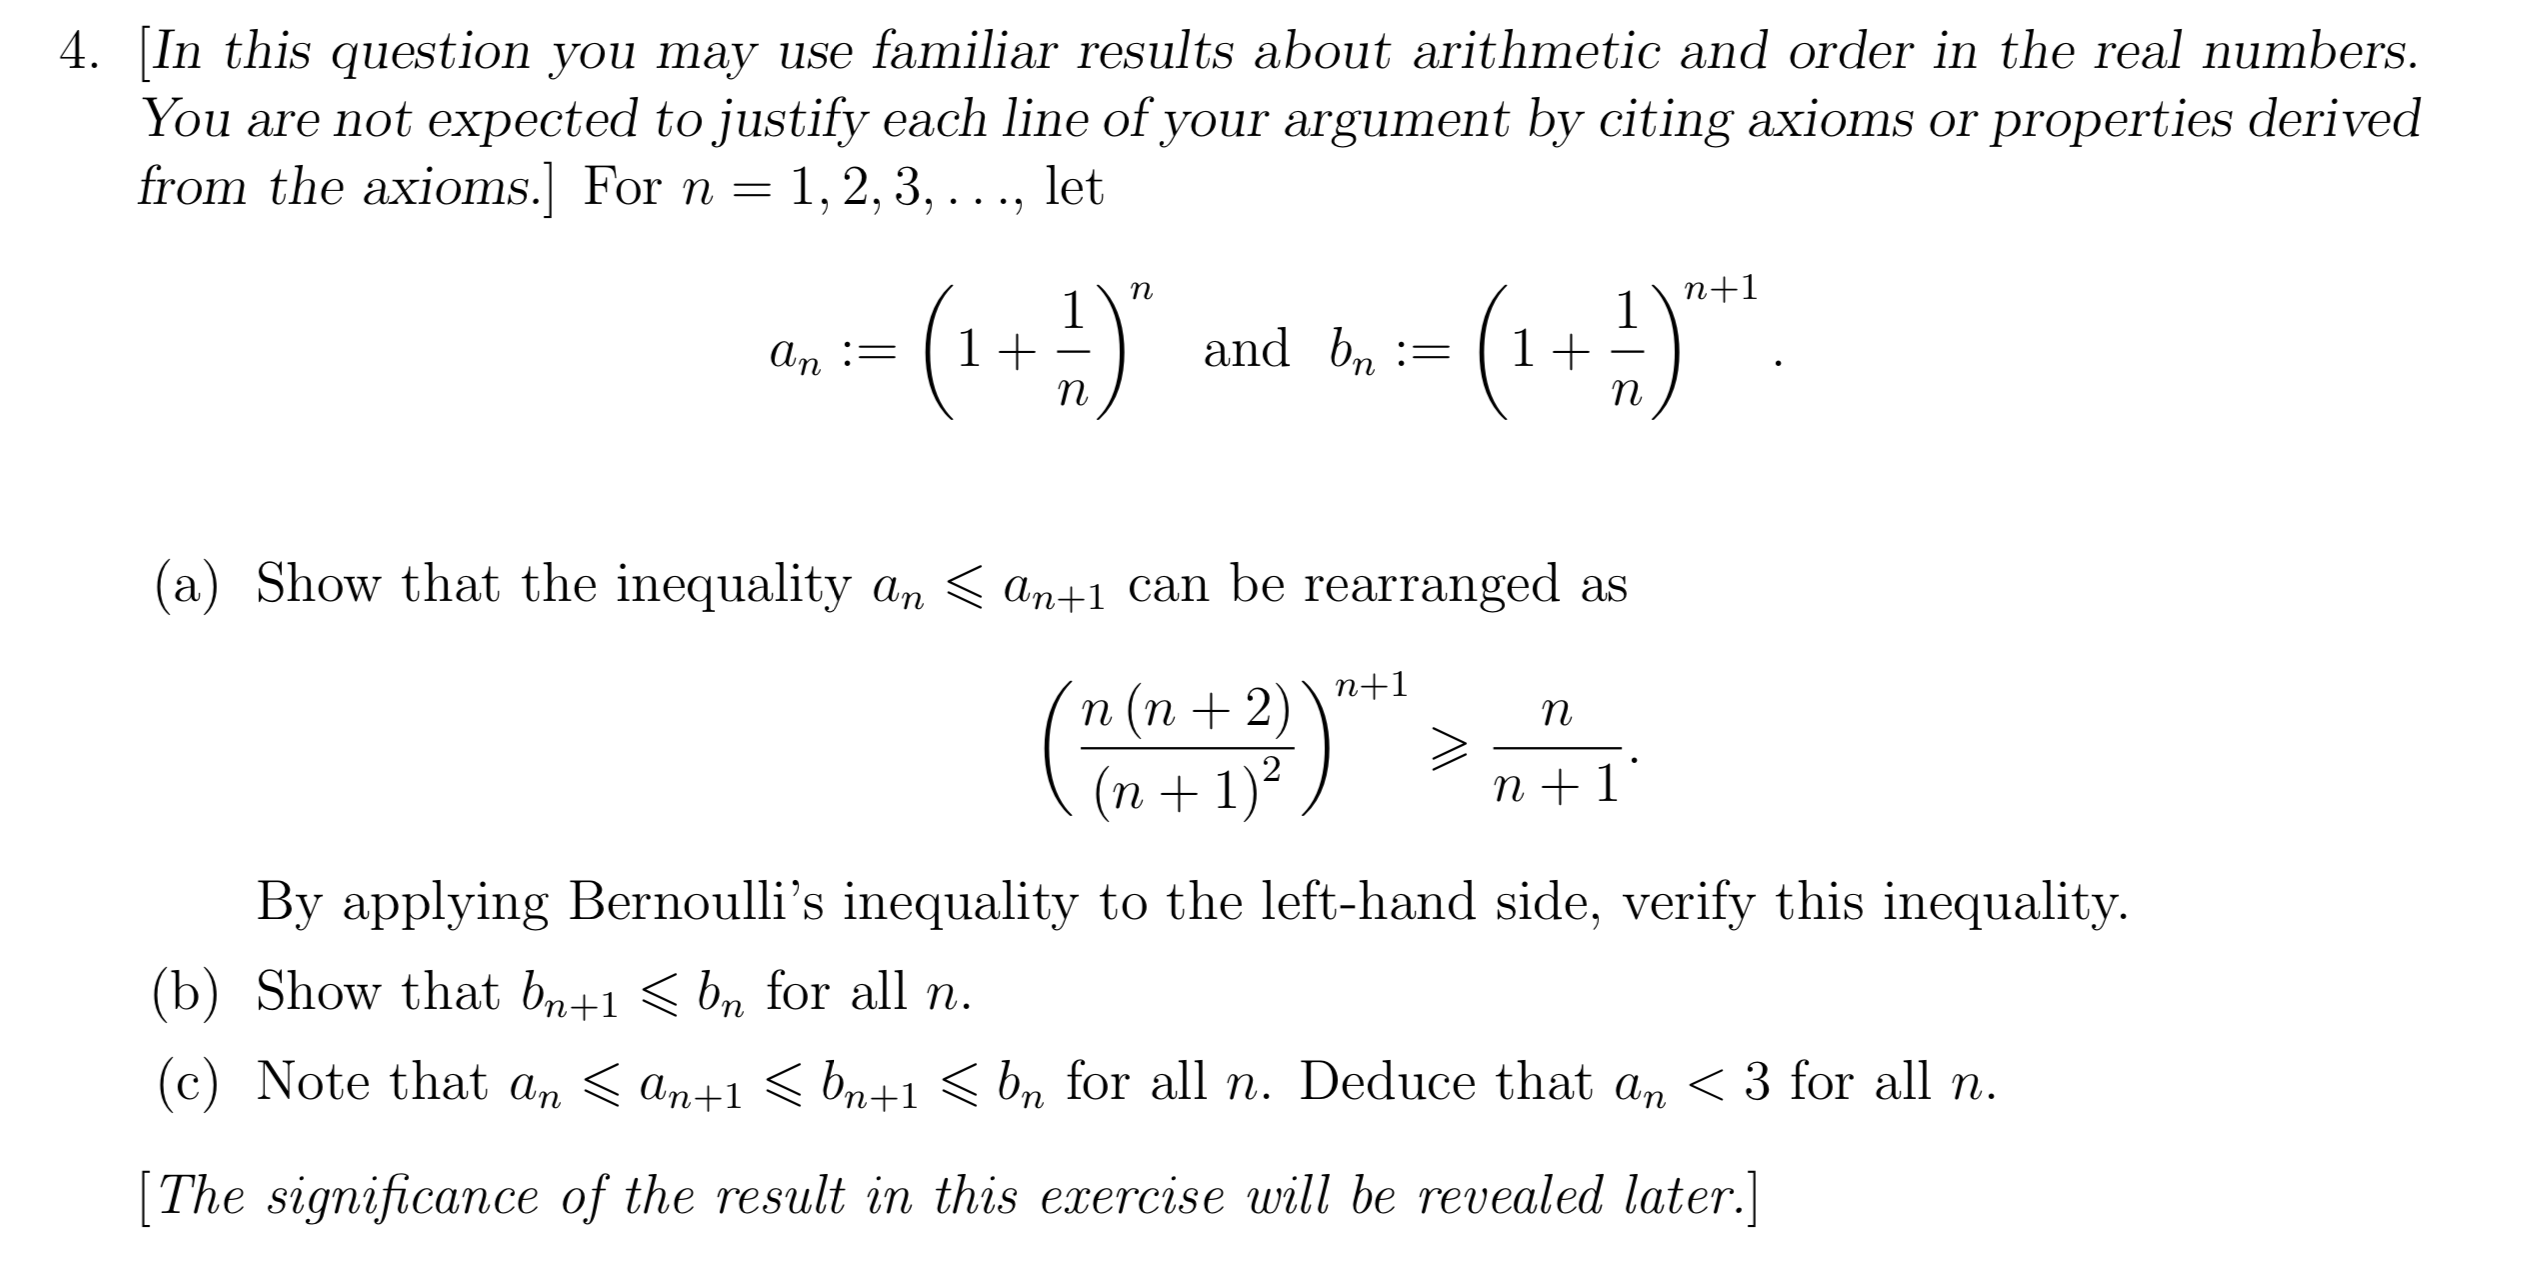
\includegraphics[width=400pt]{img/oxford-prelims-M2-analysis-I-sheet-1-4.png}
\end{mdframed}
\newpage
\subsection{}
\begin{mdframed}
  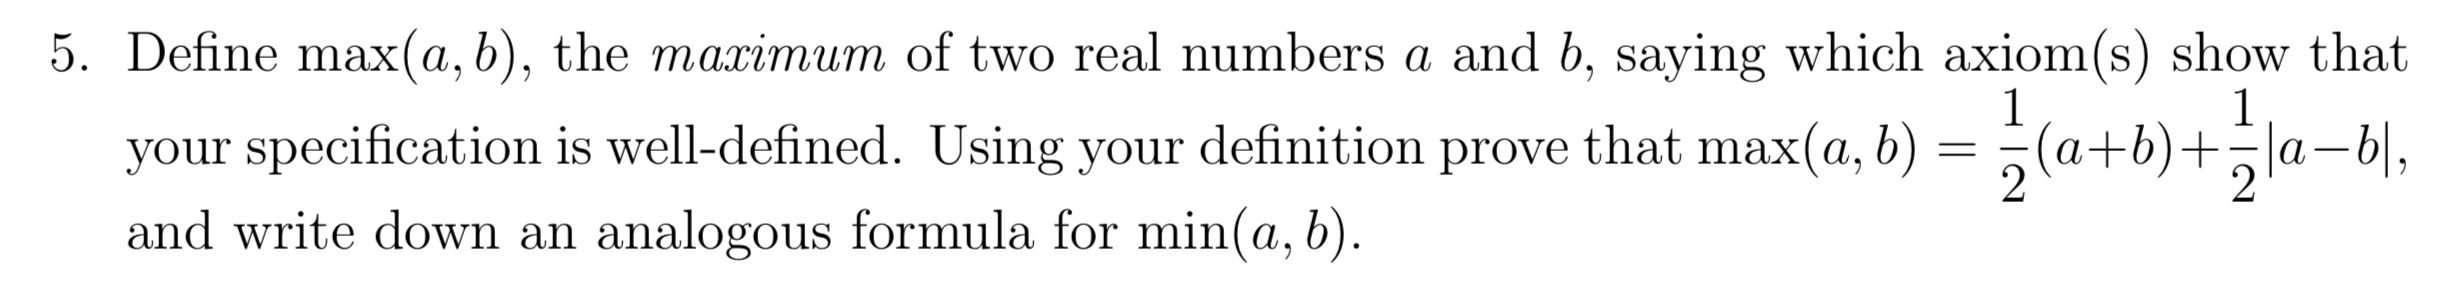
\includegraphics[width=400pt]{img/oxford-M2-analysis-I-1-5.png}
\end{mdframed}

\newpage
\section{Sheet 2}

\newpage
\subsection{}
\begin{mdframed}
  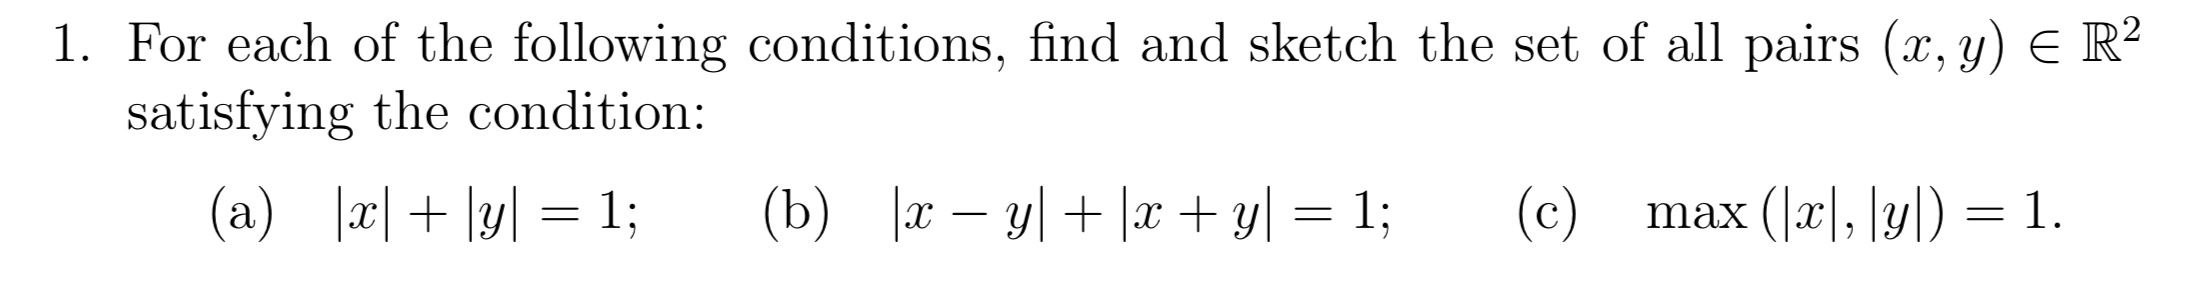
\includegraphics[width=400pt]{img/oxford-M2-analysis-I-2-1.png}
\end{mdframed}

\newpage
\subsection{}
\begin{mdframed}
  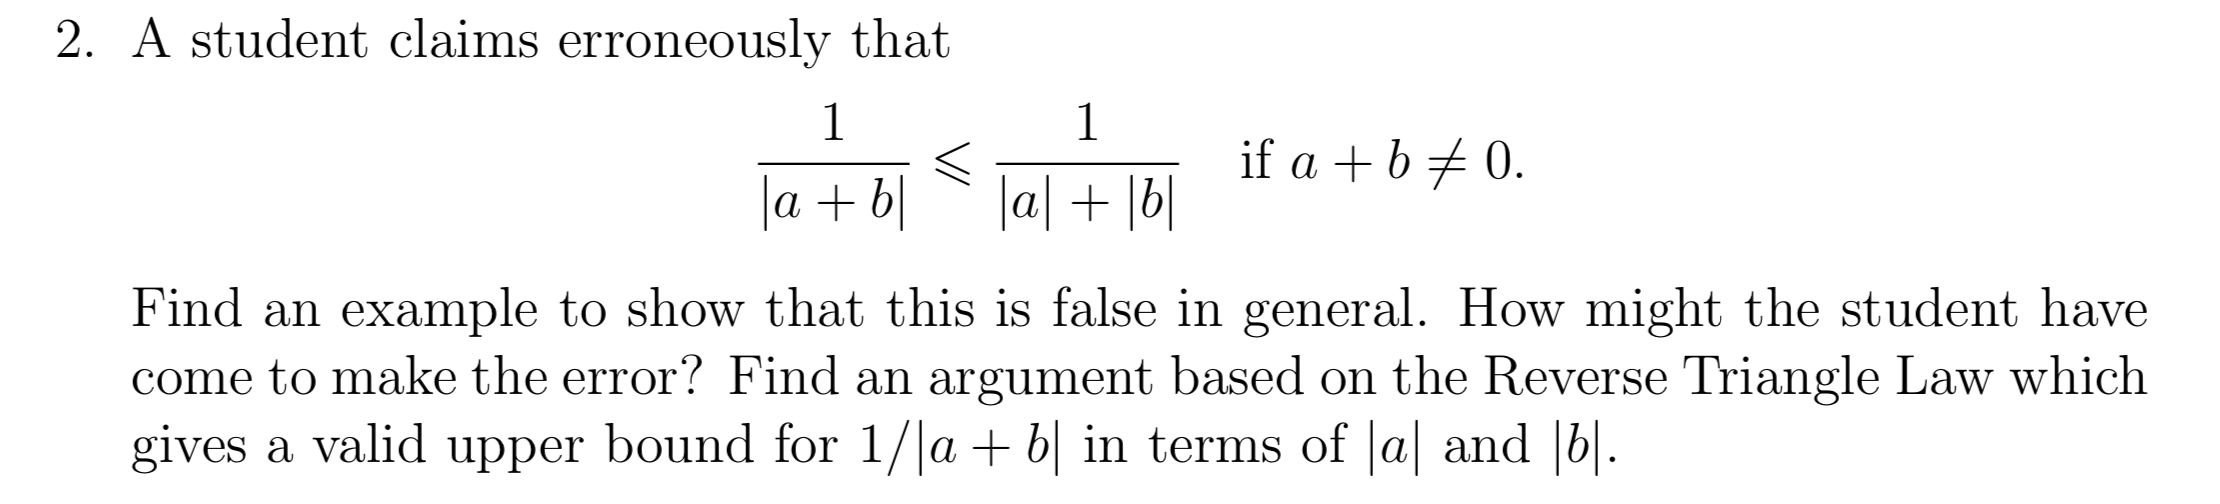
\includegraphics[width=400pt]{img/oxford-M2-analysis-I-2-2.png}
\end{mdframed}

\newpage
\subsection{(COMPLETE)}
\begin{mdframed}
  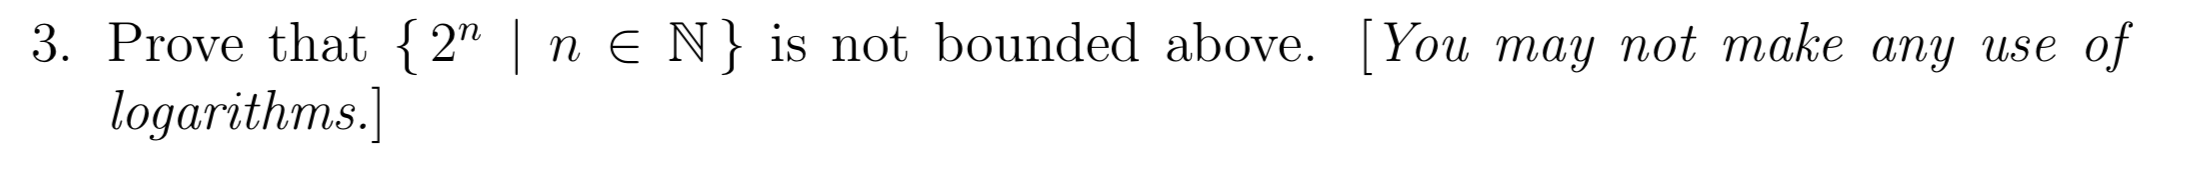
\includegraphics[width=400pt]{img/oxford-M2-analysis-I-2-3.png}
\end{mdframed}

\begin{proof}
  Let $S = \{2^n ~|~ n \in \N\}$ and suppose an upper bound for $S$ exists.

  Then $\sup S$ exists by completeness of the reals.

  By the Approximation Property there exists $2^k \in S$ such that
  \begin{align*}
    \sup S - \frac{1}{2} < 2^k \leq \sup S.
  \end{align*}
  Note that $k+1 \in \N$ therefore $2^{k+1} = 2^k + 2^k \in S$. Therefore
  \begin{align*}
    \sup S - \frac{1}{2} + 2^k &< 2^{k+1} \leq \sup S\\
    \sup S &\leq \sup S + \frac{1}{2} - 2^k < \sup S,
  \end{align*}
  a contradiction. Therefore no upper bound for $S$ exists.
\end{proof}

\newpage
\subsection{(COMPLETE)}
\begin{mdframed}
  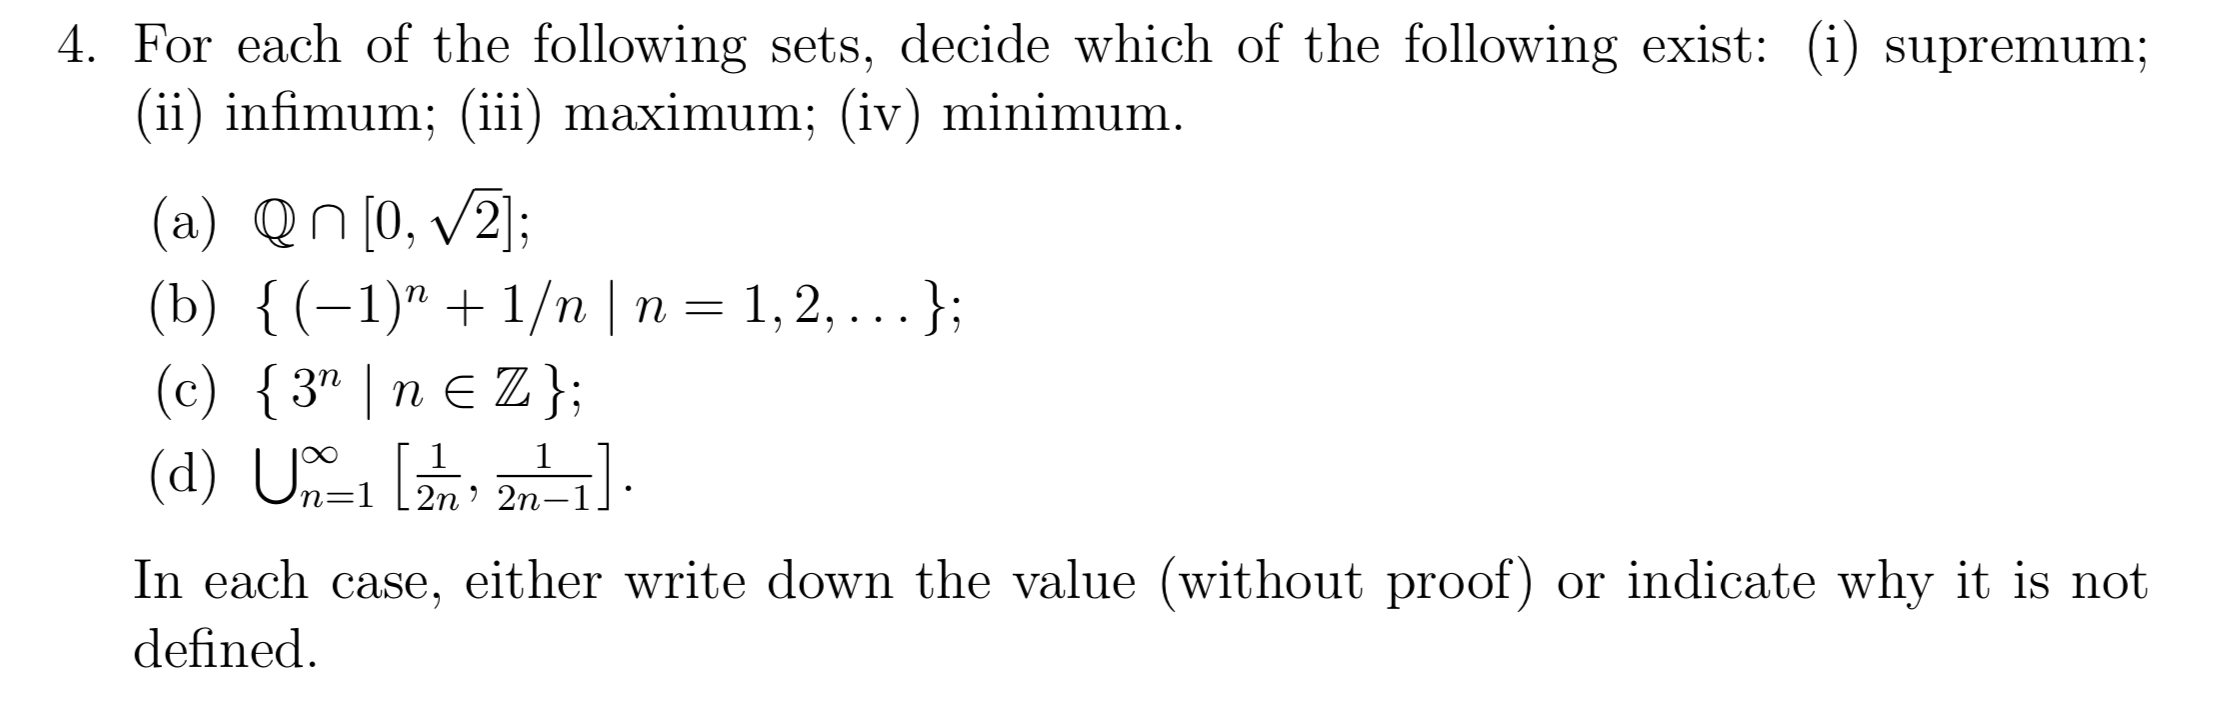
\includegraphics[width=400pt]{img/oxford-M2-analysis-I-2-4.png}
\end{mdframed}
\begin{enumerate}
\item $S = \Q \cap [0, \sqrt 2]$
  \begin{align*}
    \sup S &= \sqrt 2\\
    \max S &= \sqrt 2\\
    \min S &= 0\\
    \inf S &= 0
  \end{align*}
\item $S = \{(-1)^n + 1/n ~|~ n=1,2,\ldots\}$
  \begin{align*}
    \sup S &= 3/2\\
    \max S &= 3/2\\
    \min S ~&\text{does not exist since $\inf S \not\in S$}\\
    \inf S &= -1
  \end{align*}
\item $S = \{3^n ~|~ n \in \Z\}$
  \begin{align*}
    \sup S ~&\text{does not exist, $S$ has no upper bound}\\
    \max S ~&\text{does not exist, $S$ has no upper bound}\\
    \min S ~&\text{does not exist, $S$ has no lower bound}\\
    \inf S &= 0
  \end{align*}
\item $S = \cup_{n=1}^\infty [\frac{1}{2n}, \frac{1}{2n - 1}]$
  \begin{align*}
    \sup S ~&= 1\\
    \max S ~&= 1\\
    \min S ~&\text{does not exist, $S$ has no lower bound}\\
    \inf S ~&=0
  \end{align*}
\end{enumerate}

\newpage
\subsection{(COMPLETE)}
\begin{mdframed}
  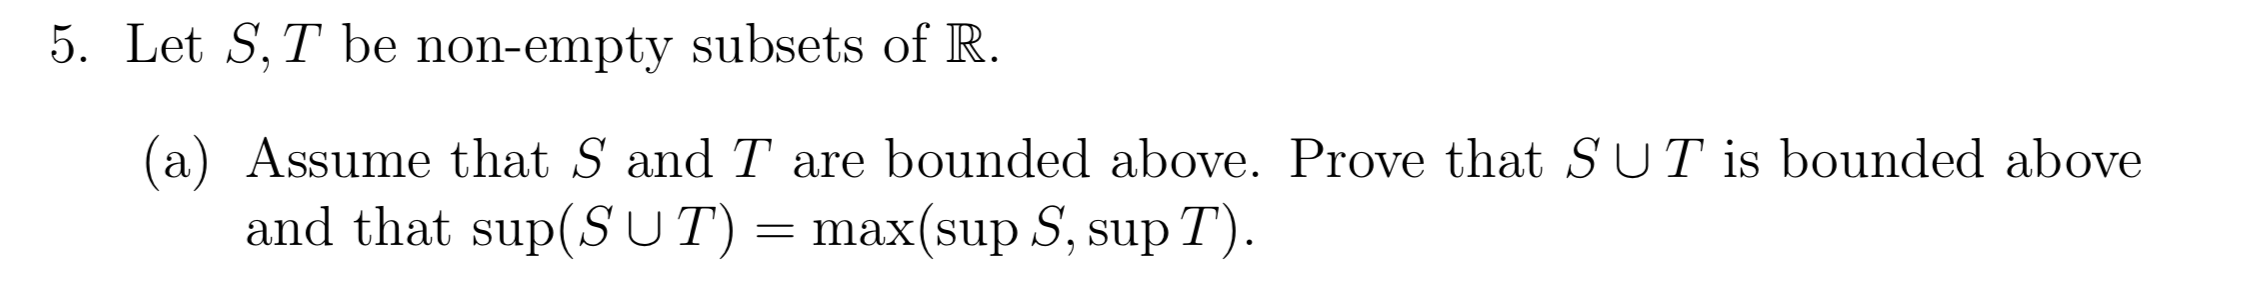
\includegraphics[width=400pt]{img/oxford-M2-analysis-I-2-5-a.png}
\end{mdframed}

\begin{proof}
  Let $S, T \subset \R$ with $S, T \neq \emptyset$. Assume that $S$ and $T$ are bounded
  above. Then $\sup S$ and $\sup T$ exist. Let $b = \max(\sup S, \sup T)$.

  Then $b \geq s$ for all $s \in S$ and $b \geq t$ for all $t \in T$. Therefore $b$ is an upper
  bound for $S \cup T$.

  Suppose there exists $a < b$ such that $a$ is an upper bound of $S \cup T$. Then either
  $a < \sup S$ or $a < \sup T$. Without loss of generality, suppose $a < \sup S$. Then $a$ is not
  an upper bound of $S$. Therefore there exists $s \in S$ such that $s > a$. But
  $s \in S \cup T$, therefore $a$ is not an upper bound of $S \cup T$, a contradiction.
\end{proof}

\begin{mdframed}
  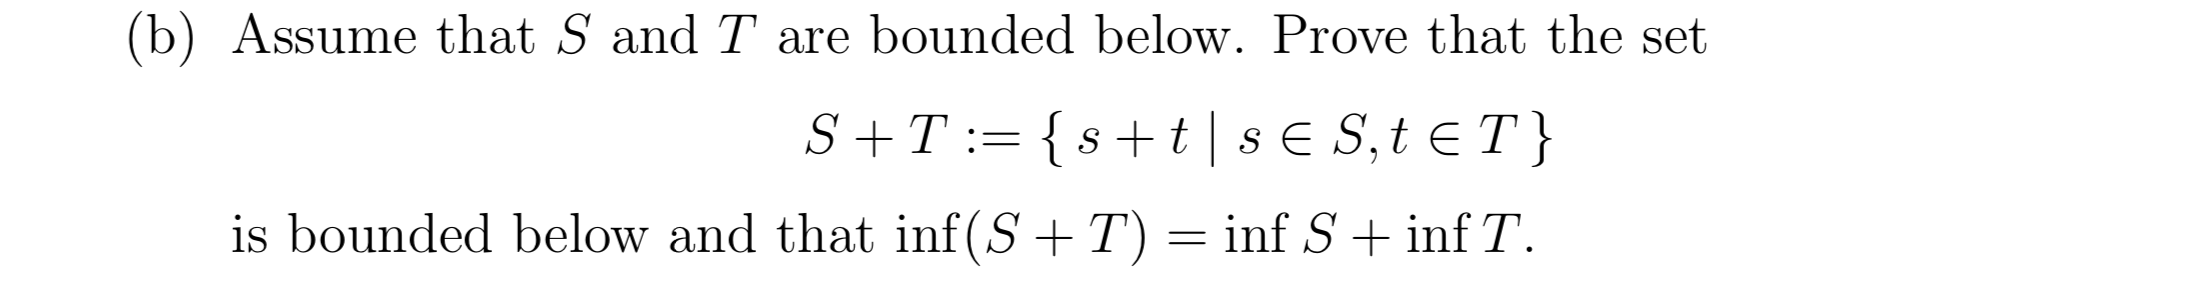
\includegraphics[width=400pt]{img/oxford-M2-analysis-I-2-5-b.png}
\end{mdframed}

\begin{proof}
  Let $S, T \subset \R$ with $S, T \neq \emptyset$. Assume that $S$ and $T$ are bounded
  below. Then $\inf S$ and $\inf T$ exist. Define
  \begin{align*}
    S + T := \{s + t ~|~ s \in S, t \in T\}.
  \end{align*}
  Let $a = \inf S + \inf T$.

  We claim that $a$ is a lower bound for $S + T$, i.e. $u \geq a$ for all $u \in S + T$.

  Let $u \in S + T$. Then $u = s + t$ for some $s \in S, t \in T$. Therefore
  $$u = (\inf S + v) + (\inf T + w) = a + (v + w) \geq a$$ for some $v, w \geq 0$. Therefore $a$ is
  a lower bound for $S + T$ as claimed.

  We further claim that $a = \inf S + T$.

  Suppose for a contradiction that there exists $b > a$ such that $b$ is a lower bound for
  $S + T$. Then $$b = a + v + w = (\inf S + v) + (\inf T + w)$$ for some $v, w > 0$. Fix
  $0 < \delta < \min(v, w)$. By {\bf 4.9} (Approximation Property of the supremum/infimum) there
  exist $s \in S$ and $t \in T$ such that $\inf S \leq s < \inf S + \delta$ and
  $\inf T \leq t < \inf T + \delta$. But then $s + t \in S + T$ and $s + t < b$, so $b$ is not a
  lower bound for $S + T$, a contradiction. Therefore $a = \inf S + T$ as claimed.
\end{proof}

\newpage
\subsection{}
\begin{mdframed}
  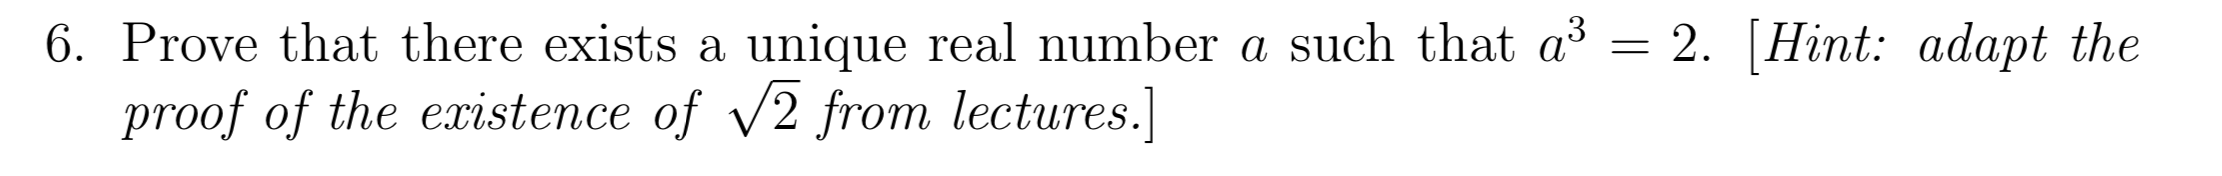
\includegraphics[width=400pt]{img/oxford-M2-analysis-I-2-6.png}
\end{mdframed}

\begin{proof}
  Let $S = \{x \in \R ~|~ x^3 < 2\}$. Since $S$ is bounded above, $\sup S$ exists. Let
  $a = \sup S$. By trichotomy it suffices to show that $a^3 < 2$ and $a^3 > 2$ lead to
  contradictions.

  First suppose $a^3 < 2$. We seek $h > 0$ such that $(a + h)^3 < 2$ since then $a + h \in S$,
  which would contradict the definition $a := \sup S$. Note that
  \begin{align*}
    (a + h)^3 &= a^3 + 3a^2h + 3ah^2 + h^3 - 2\\
              &< a^3 + 7a^2h - 2 ~~~~~~~~~~~~~~~~~~~~~~~~\text{if $h < a$}\\
              &< 0              ~~~~~~~~~~~~~~~~~~~~~~~~~~~~~~~~~~~~~~~~~\text{if $h < \frac{2 - a^3}{7a^2}$},
  \end{align*}
  therefore if we take $h < \min\(a, \frac{2 - a^3}{7a^2}\)$ then we have the desired
  contradiction.

  Alternatively suppose that $a^3 > 2$. By the Approximation Property for all $0 < h < a$ we can
  find $s \in S$ such that $a - h < s$, therefore $(a - h)^3 < s^3$. We seek an $h$ for which
  $(a - h)^3 > 2$ since then we would have $s^3 > 2$ which would contradict the definition of
  $S$. Note that
  \begin{align*}
    (a - h)^3 - 2 &= a^3 - 3a^2h + 3ah^2 - h^3 - 2\\
                  &> 0 ~~~~~~~~~~~~~~~~~~~~~~~~~~~~~~~~~~~~~~~~~\text{if $3ah^2 > 3a^2h + h^3$}.
  \end{align*}
  So we require $3ah > 3a^2 + h^2 \iff 3a^2 - 3ah + h^2 < 0$.

  \red{Incomplete}
\end{proof}

\newpage
\subsection{}
\begin{mdframed}
  
\includegraphics[width=400pt]{img/oxford-M2-analysis-I-2-7-a.png}
\end{mdframed}
\begin{definition*}[Countable]
  A set $S$ is countable if $S \preceq N$. I.e. there exists an injection $f:S \to \N$.
\end{definition*}
\begin{definition*}[Uncountable]
  A set $S$ is uncountable if it is not countable.
\end{definition*}
\begin{definition*}[Injection]
  A function $A \to B$ is an injection if $f(a_1) = f(a_2) \implies a_1 = a_2$.
\end{definition*}
\begin{proof}
  Suppose for a contradiction that $\R \setminus \Q$ is countable. Then an injection
  $f:\R \setminus \Q \to \N$ exists. Since $\Q$ is countable, an injection $g:\Q \to \N$
  exists. Consider the function $h:\R \to \N$ defined by
  \begin{align*}
    h(x) =
    \begin{cases}
      2f(x) &x \in \R \setminus \Q\\
      2g(x) + 1 &x \in \Q.
    \end{cases}
  \end{align*}
  We claim that $h:\R \to \N$ is an injection. Note that
  \begin{enumerate}[label=(\roman*)]
  \item $h(\R\setminus\Q) \cap h(\Q) = \emptyset$
  \item The $\R \to \R$ functions defined by $x \mapsto 2x$ and $x \mapsto 2x + 1$ are both
    injections.
  \item The composition of two injections is an injection.
  \end{enumerate}
  Suppose $h(x_1) = h(x_2)$. Then either $x_1, x_2 \in \Q$ or $x_1, x_2 \in \R\setminus\Q$ by
  (i). In both cases we have $x_1 = x_2$ by (ii) and (iii). Therefore $h:\R \to \N$ is an
  injection, hence $\R$ is countable.

  But $\R$ is not countable, so we have a contradiction. Therefore no such injection $f$ exists,
  i.e. $\R\setminus\Q$ is uncountable.
\end{proof}

\begin{mdframed}
  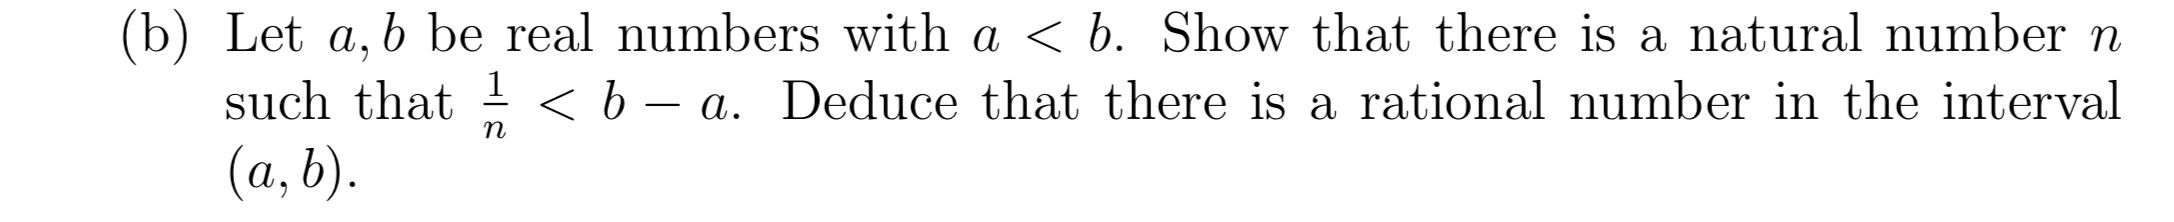
\includegraphics[width=400pt]{img/oxford-M2-analysis-I-2-7-b.png}
\end{mdframed}

\begin{proof}
  Let $a, b$ be real numbers with $a < b$. Then $b - a > 0$. Since $\N$ is not bounded above
  (Archimedean property) there exists $n \in \N$ such that $n > 1/(b - a)$, therefore
  $1/n < b - a$.

  Suppose $a$ is rational. Then $a + 1/n \in (a, b)$ is rational. Similarly, if $b$ is rational
  then $b - 1/n \in (a, b)$ is rational.

  Finally, suppose neither $a$ nor $b$ are rational. \red{How to prove this case?}
\end{proof}

\begin{mdframed}
  
\includegraphics[width=400pt]{img/oxford-M2-analysis-I-2-7-c.png}
\end{mdframed}

Let $a, b$ be real numbers with $a < b$.

\newpage
\subsection{}
\begin{mdframed}
  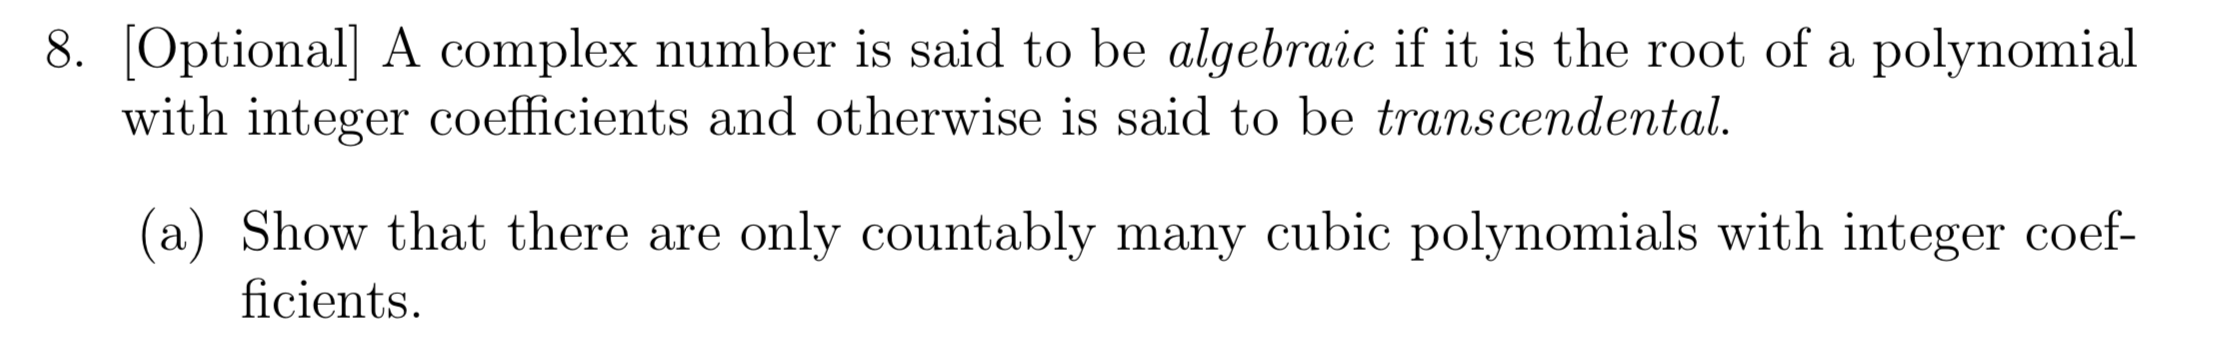
\includegraphics[width=400pt]{img/oxford-M2-analysis-I-2-8-a.png}
\end{mdframed}

\begin{proof}
  The cardinality of the set of cubic polynomials with integer coefficients is equal to the
  cardinality of the set
  $A := \{(a, b, c, d) ~|~ a, b, c, d \in \Z, a \neq 0\} = \(\Z\setminus\{0\}\) \times \Z^3$.

  Let $f:(\Z\setminus\{0\} \times \Z^3) \to \N$ be given by $f(a, b, c, d) = 2^a3^b5^c7^d$. Then
  $f$ is an injection by uniqueness of prime factorization of the integers. Therefore $A$ is
  countable.
\end{proof}

\begin{mdframed}
  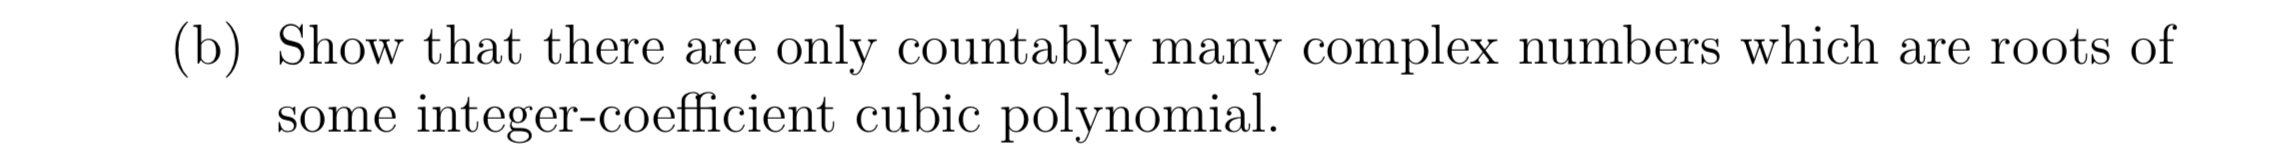
\includegraphics[width=400pt]{img/oxford-M2-analysis-I-2-8-b.png}
\end{mdframed}

\begin{proof}
  Note that a cubic polynomial has at most 3 distinct roots. Let $U$ be the set of complex
  numbers that are roots of some integer-coefficient cubic polynomial. For each such polynomial,
  assign a distinct label from $\{0, 1, 2\}$ to each of the distinct roots. Then the cardinality
  of $U$ is equal(*) to the cardinality of $B := \Z\setminus\{0\} \times \Z^3 \times \{0, 1,
  2\}$. The set $B$ is countable since $f:T \to \N$ given by
  $f(a, b, c, d, e) = 2^a3^b5^c7^d11^e$ is an injection. (\red{* How to properly deal with the fact
    that $U$ is smaller than $B$ due to some polynomials having fewer than 3 distinct roots?})
\end{proof}

\begin{mdframed}
  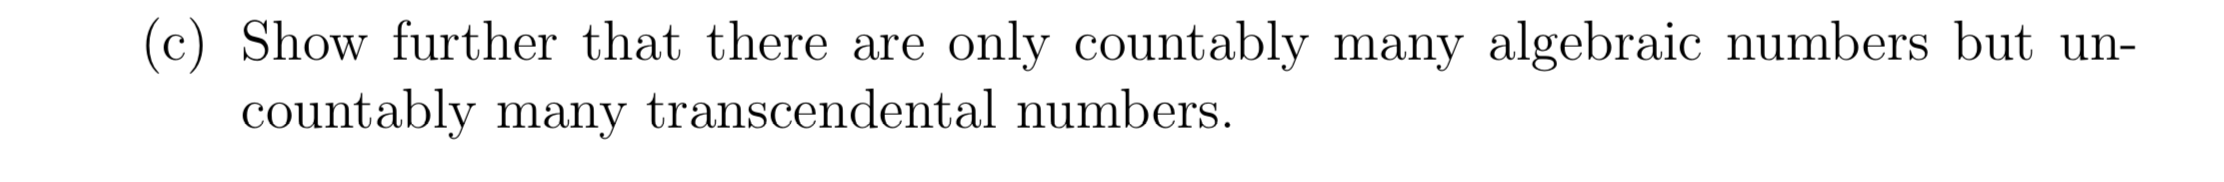
\includegraphics[width=400pt]{img/oxford-M2-analysis-I-2-8-c.png}
\end{mdframed}

\begin{proof}
  (This differs because whereas previously we were restricted to cubics, now the polynomials can
  be of any degree $n \in \N$.)

  The cardinality of the set of algebraic numbers is \red{Incomplete}.
\end{proof}

\end{document}